\subsection{Visualizations}
\label{sec:visualization}

In \cref{sec:analysis} we explored the available data and made interesting observations by looking at the numbers themselves and comparing them in a simple tabular form or with basic box plot diagrams. While this provided good insights, we as humans tend to comprehend visualizations better than raw numbers, especially for huge data sets with millions of entries such as the one on hand \autocite[2]{ware-2019}. Therefore, the following section presents and discussed some visualizations which aim to show the collected delay data in a way that is easy to understand while still providing the reader with valuable information. Specifically, the first visualizations show colored dots on a map of Vienna, with the colors representing the delay rates of those stations. Next, we present line graphs showing the variation in punctuality rate and number of departures throughout the day, separated by weekdays and weekends.

\subsubsection{Stations colored by punctuality rate}

\begin{figure}[h]
	\centering
	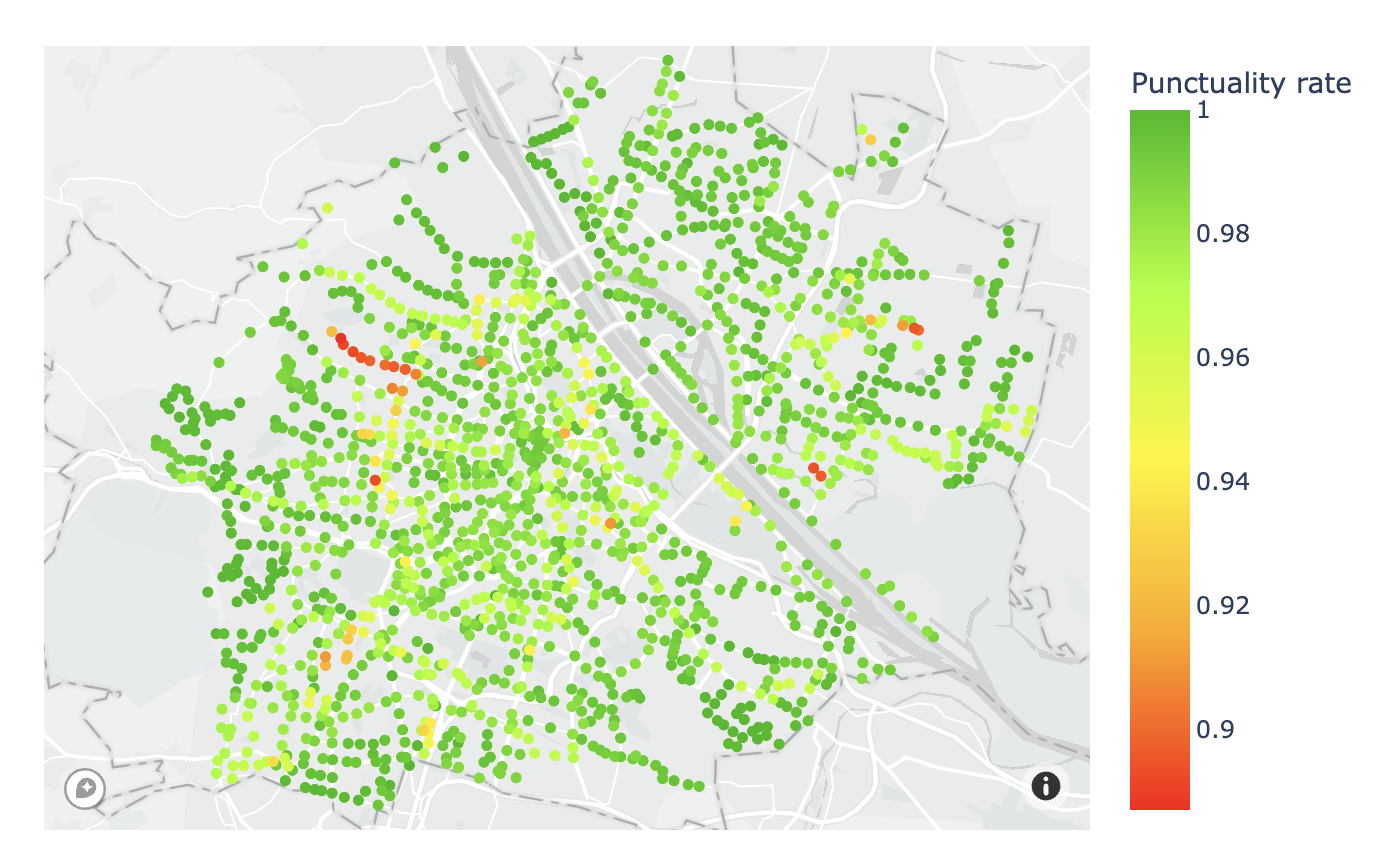
\includegraphics[width=1\textwidth]{overall-no-blaasstr}
	\caption{All stations colored by punctuality rate}
	\label{fig:overall-stations}
\end{figure}

For the first visualization, depicted in \cref{fig:overall-stations}, all stations of the network were marked with a dot at their respective location on a map of Vienna. Then, stations were colored based on their individual punctuality rate, ranging from green for a rate of 100\% to red representing a rate of 88.7\%. Since the station \textit{Blaasstraße} was already detected as an outlier in \cref{sec:analysis}, it is not included in this map as it would shift all other stations relatively far up on the color scale, resulting in an all-green map. At first glance, one can see a very good overall state, with a vast majority of stations colored light to dark green. Besides a few red spots, there is a noticeable sequence of orange and red stations, located in the northwest of the city center which all belong to bus line 42A. Besides these more delayed areas, the darkest green and thus most punctual sequences of stations can be seen on the edges of the network, most notably in the west and south of the city, in addition to the area east of the Danube River.

\begin{figure}[h]
	\centering
	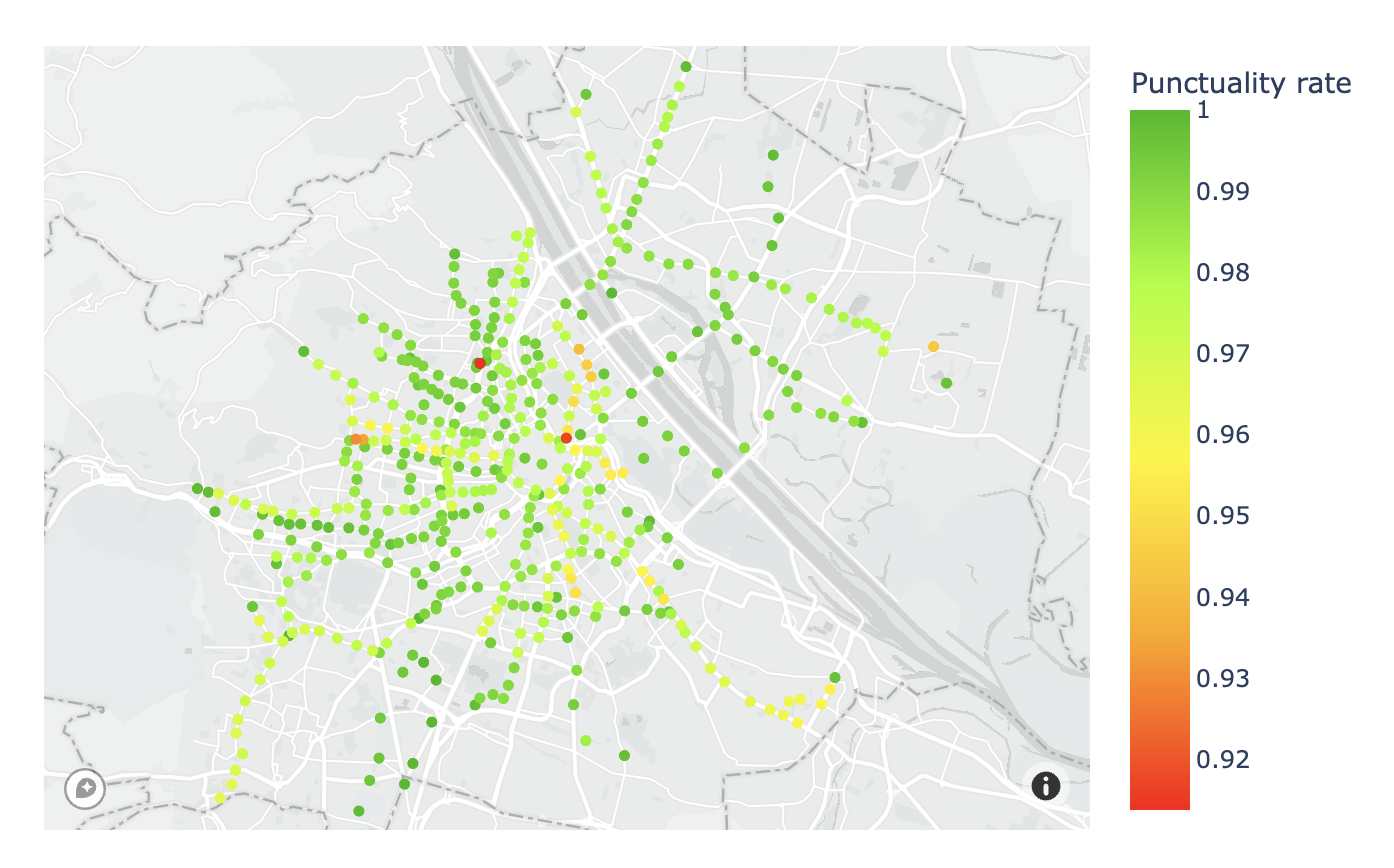
\includegraphics[width=1\textwidth]{no-buses}
	\caption{Metro and tram stations colored by punctuality rate}
	\label{fig:no-buses-stations}
\end{figure}

\begin{figure}[h]
	\centering
	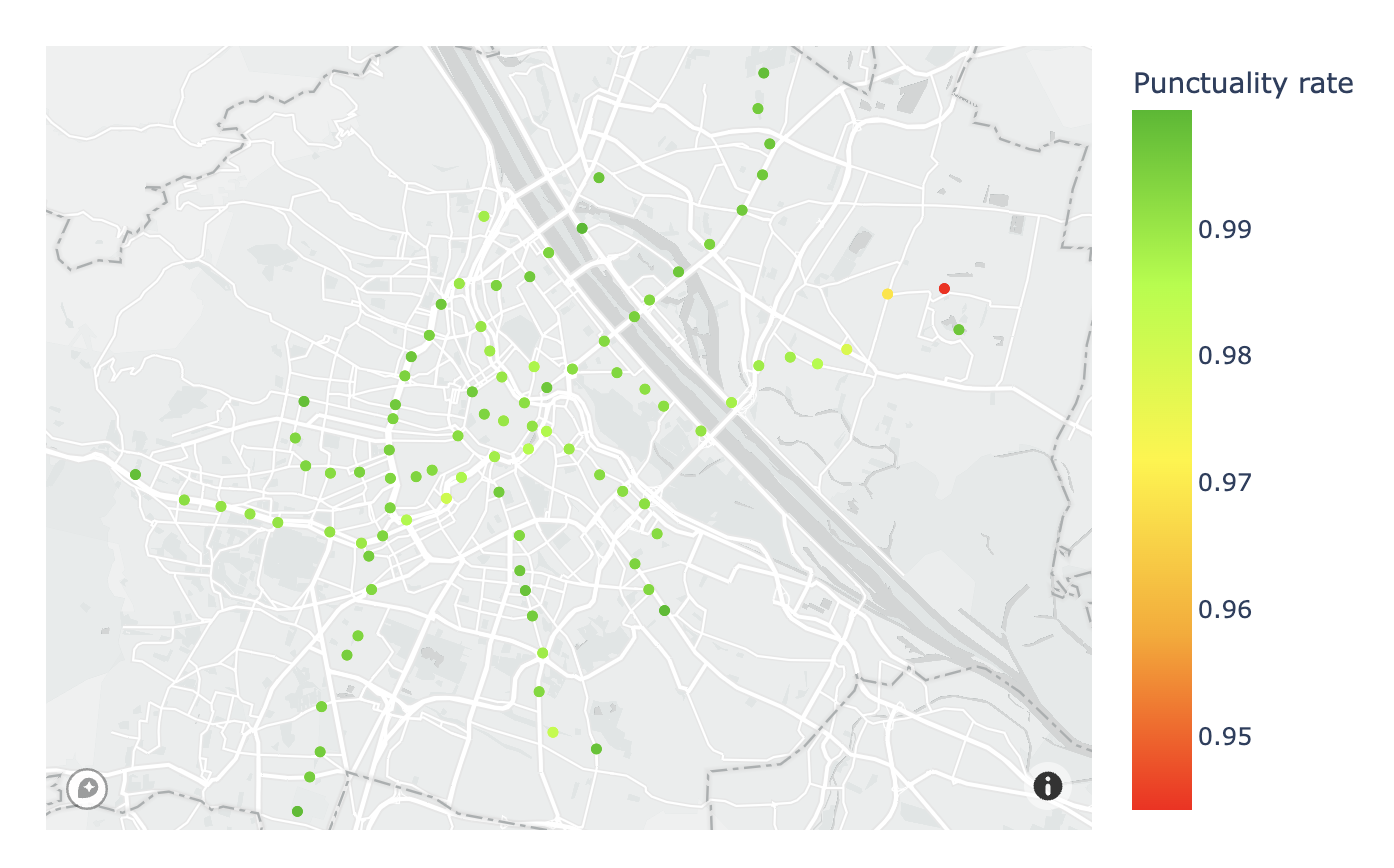
\includegraphics[width=1\textwidth]{metro-only}
	\caption{Metro stations colored by punctuality rate}
	\label{fig:metro-only-stations}
\end{figure}

Since the previous map with all bus, tram and metro stations is rather dense, \cref{fig:no-buses-stations} shows only tram and metro stations. On there, one can see two red dots, which are the stations \textit{Marsanogasse} located north of the city center and \textit{Gredlerstraße} which is right in the center. Besides these two stations, the most delayed tram lines are visible on the map because of their more yellow-colored stations. For example, line 71 goes from the center to the southeast and line 2 starts north of the city center and continues west. The most punctual regions this time are located in the west, which follows the fact that there are significantly more tram and metro stations in this area.

\Cref{fig:metro-only-stations} goes one step further and shows metro stations only, which allows an even more nuanced analysis. The map becomes once again significantly less densely dotted, with only 96 metro stations remaining. Almost all stations are green, confirming results from \cref{sec:analysis} that metro lines generally have high punctuality rates. The two exceptions are the stations \textit{Hausfeldstraße} and \textit{Aspern Nord} located on the far-east, which are both part of metro line U2. Interestingly, the next station after the red-colored \textit{Aspern Nord} shows a dark shade of green and therefore a high punctuality rate.

\subsubsection{Punctuality rate by time of day}

Until now, we have always analyzed all departures during the entire collection period of 30 days. However, another interesting aspect is the correlation of punctuality to the time of day. During rush hours in the morning and evening, higher delay rates are expected. In order to see this effect, all departures were grouped by the hour they were scheduled, ranging from 0 to 23. Furthermore, an additional separation between weekdays and weekends was done in order to capture the effect of rush hour traffic better. \Cref{fig:time-of-day-weekday} shows departures from Monday to Friday while \cref{fig:time-of-day-weekend} shows departures that occurred on Saturdays and Sundays.

\begin{figure}[h]
	\centering
	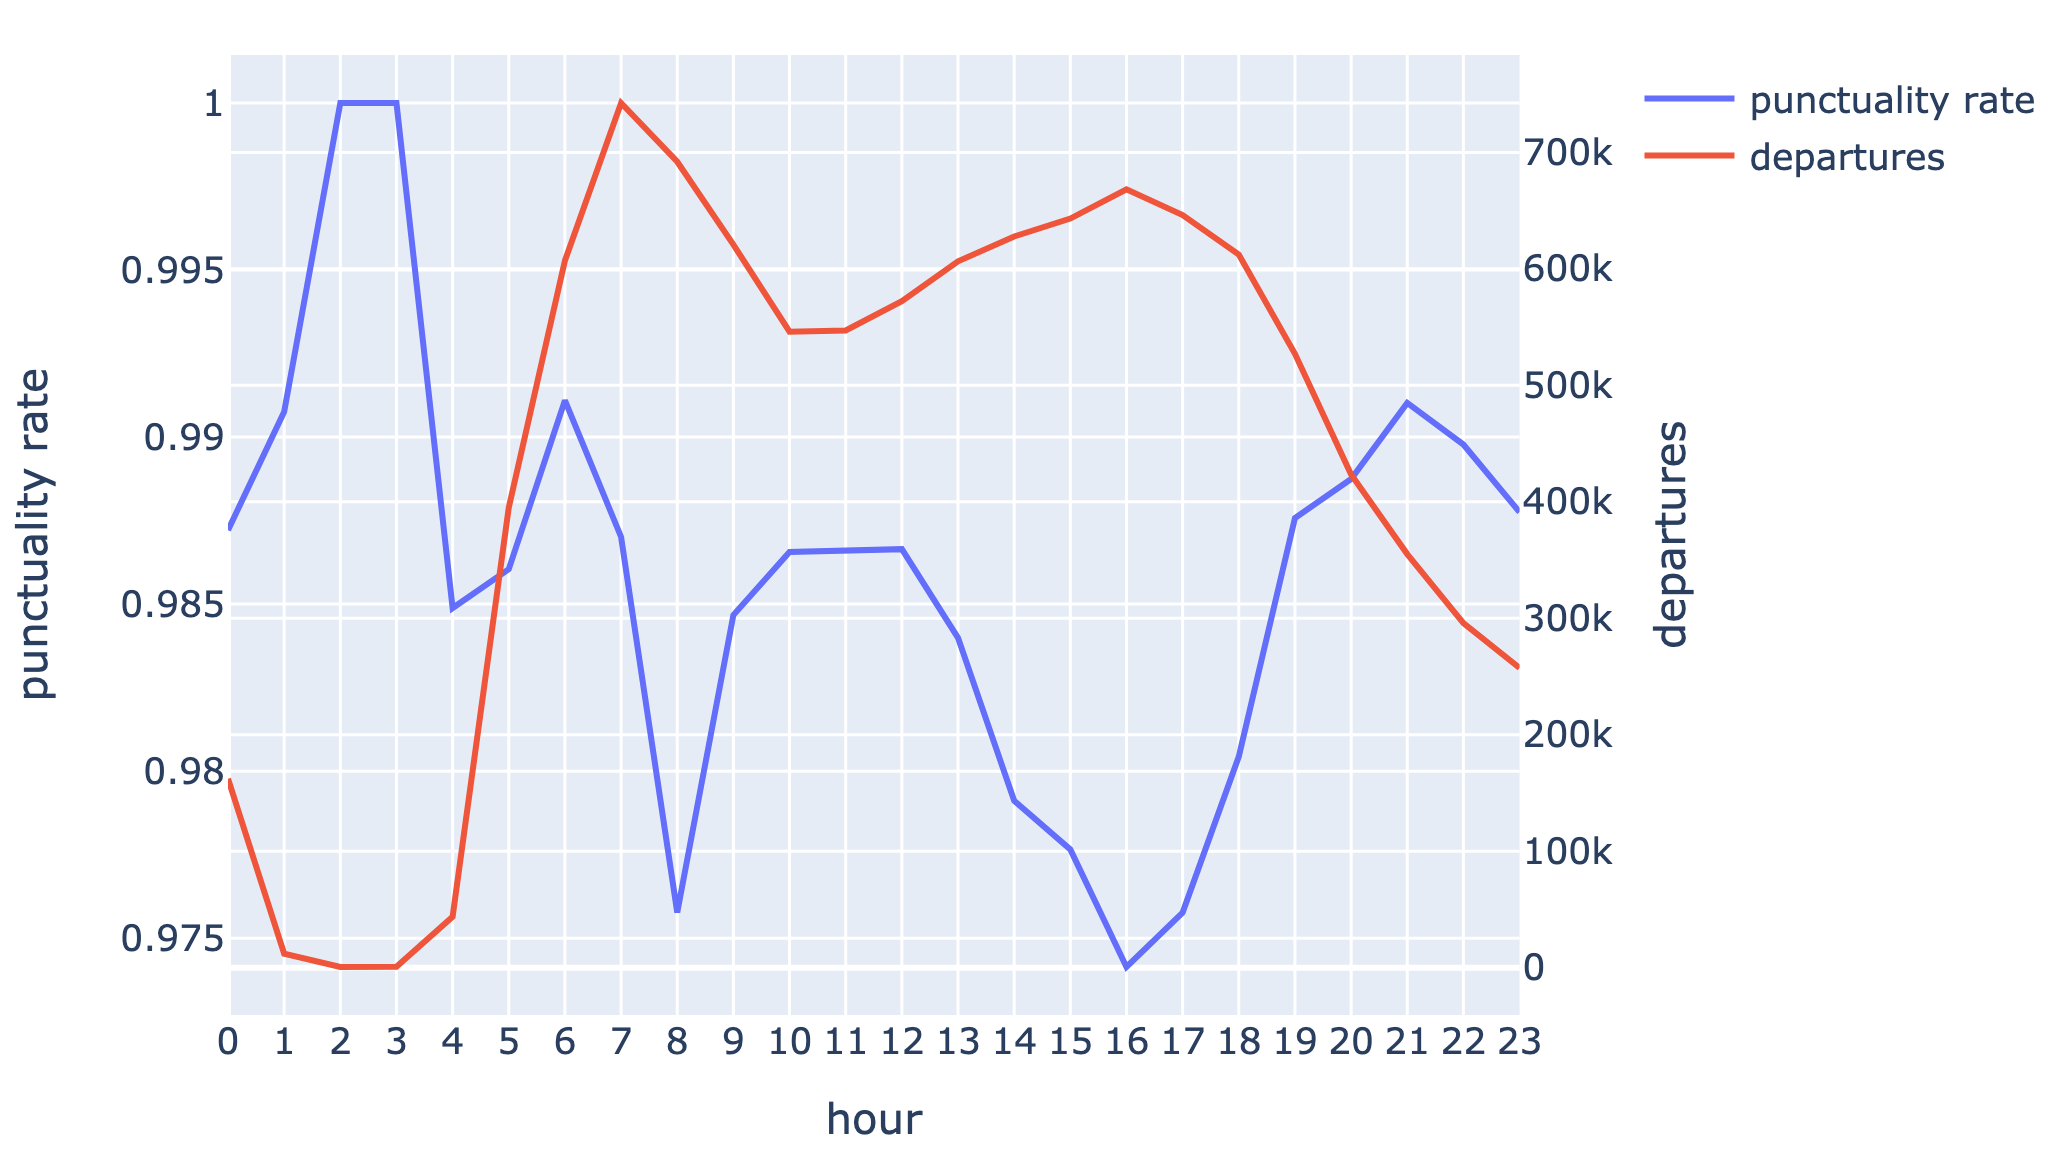
\includegraphics[width=1\textwidth]{time-of-day-weekday}
	\caption{Punctuality rate and number of departures by time of day on weekdays}
	\label{fig:time-of-day-weekday}
\end{figure}

\begin{figure}[h]
	\centering
	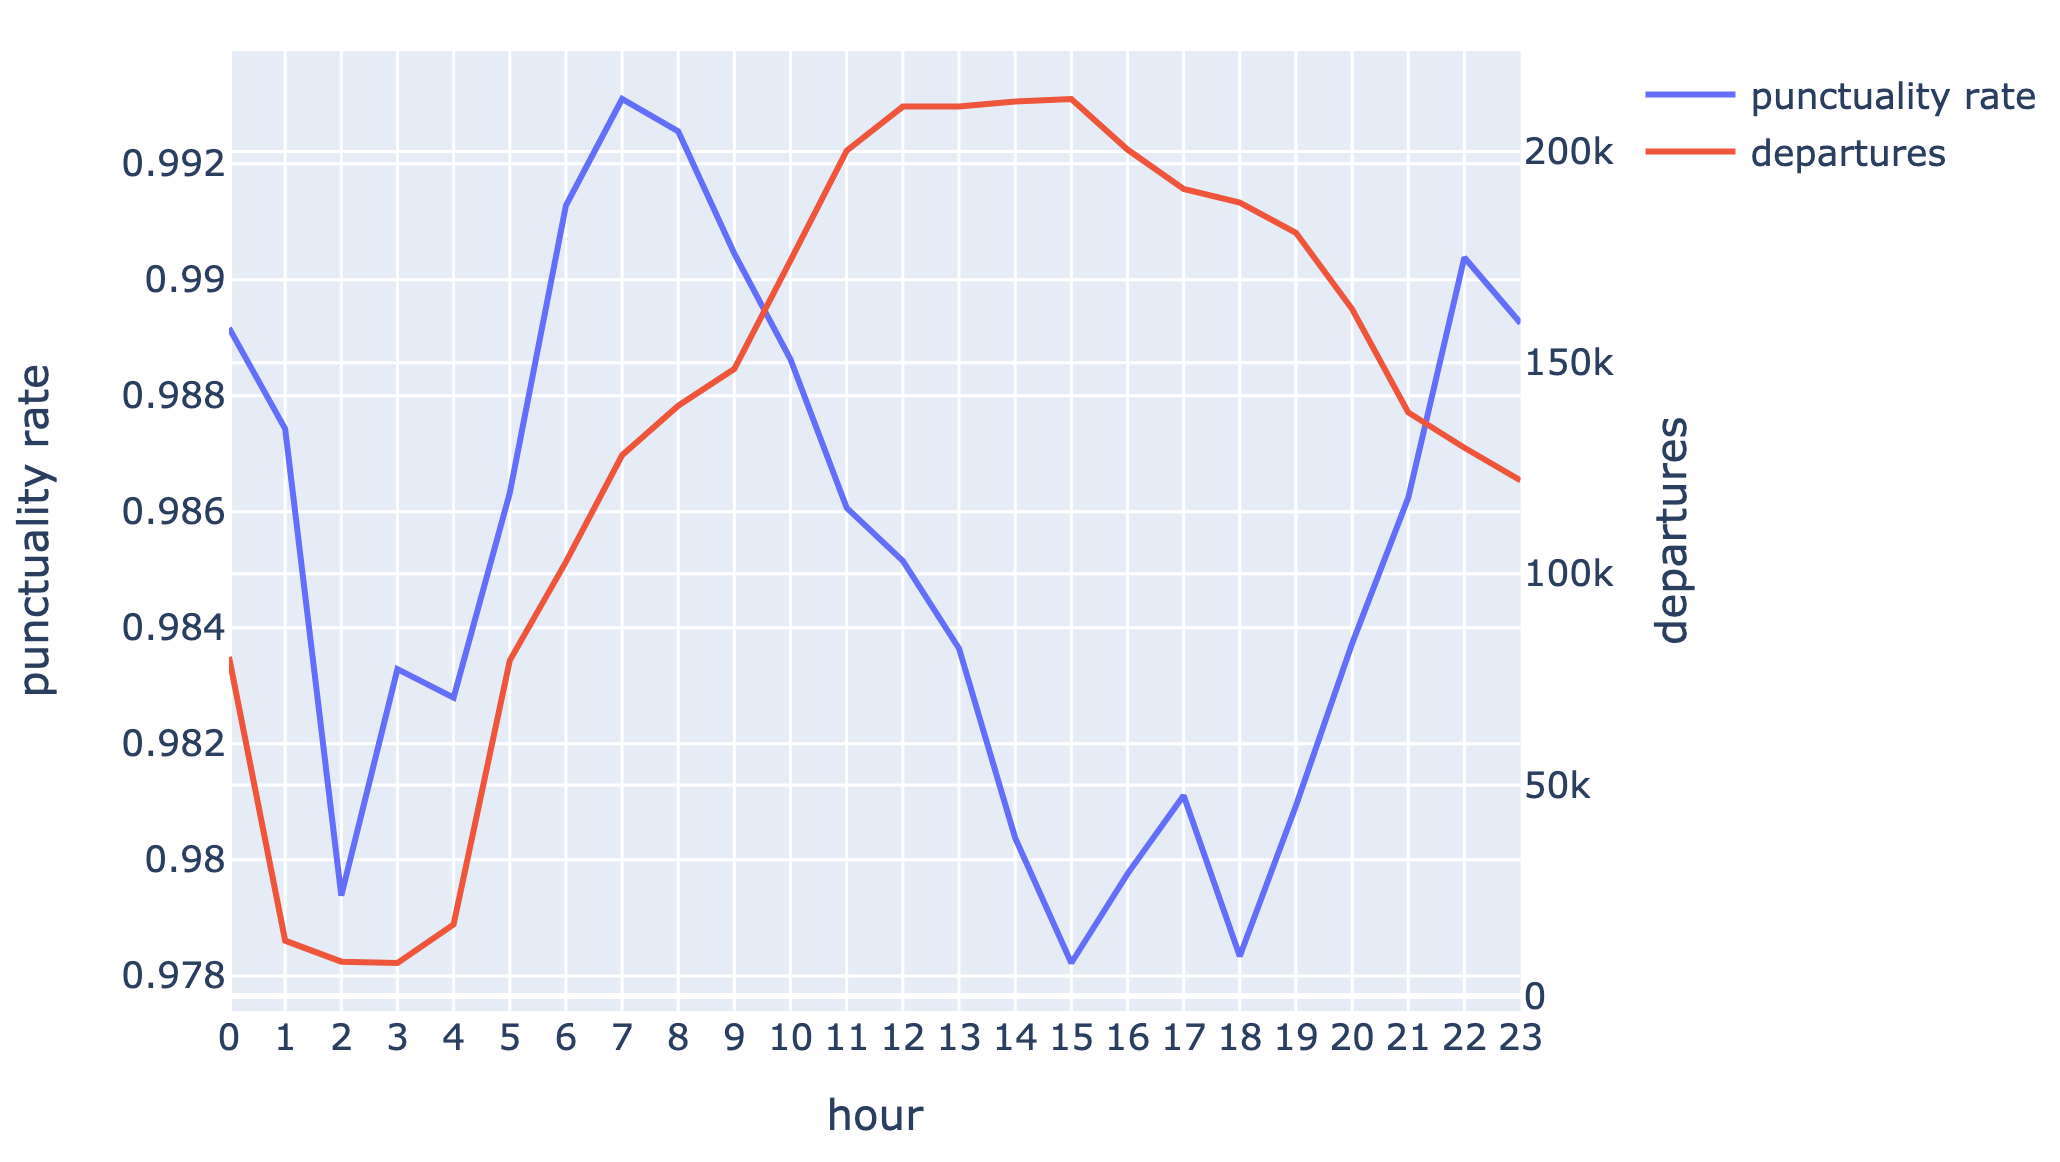
\includegraphics[width=1\textwidth]{time-of-day-weekend}
	\caption{Punctuality rate and number of departures by time of day on weekends}
	\label{fig:time-of-day-weekend}
\end{figure}

For weekdays, the punctuality rate drops significantly at \DTMtime{08:00:00} and \DTMtime{16:00:00}. During this timeframe, the number of departures also rises to the highest points, peaking at \DTMtime{07:00:00} and \DTMtime{16:00:00} with around 750,000 and 670,000 departures per hour respectively. While the amount of departures stays relatively high during midday, the punctuality rate recovers significantly. From \DTMtime{02:00:00} to \DTMtime{03:00:00} in the night, punctuality even reaches 100\%. However, on weekdays there are only limited services with only a few bus lines running, shown by the number of departures which drop to around 8000 per hour. On weekends, the image differs a lot and shows that the number of departures rises during the morning and reaches its highest point at noon, going back down at \DTMtime{15:00:00}. Further, those peaks are notably lower than on weekdays, reaching less than a third of departures with around 220,000. The punctuality rate behaves very differently too, with its lowest values being at \DTMtime{02:00:00} and \DTMtime{15:00:00}, this time reaching its maximum at \DTMtime{07:00:00}.